%\documentclass{sig-alternate-05-2015}
\documentclass[conference]{IEEEtran_custom}

\pdfoutput=1 % Force arXiv to use PDFLaTeX

\usepackage{multicol}
\usepackage{multirow}
\usepackage{comment}
\usepackage{amssymb,amsmath, amsfonts}
\usepackage{array}
\usepackage[hidelinks]{hyperref}
\usepackage{epsfig}
\usepackage{graphicx}
\usepackage{tabularx}
\usepackage{booktabs}
\usepackage{xspace} % Used for managing spaces after defined symbols
\usepackage{flushend}
\usepackage{color}
\usepackage[numbers]{natbib}
\usepackage{textcomp}

\usepackage{subcaption}

 \usepackage{float}

\usepackage[textsize=scriptsize]{todonotes}

% configure TODONOTES
\setlength{\marginparsep}{0.1cm}
\setlength{\marginparwidth}{1.75cm}
\newcommand{\todonh}[1]{\todo[fancyline,color=green!40]{MW: #1}}
\newcommand{\todoinnh}[1]{\todo[inline,color=green!40]{MW: #1}}
\newcommand{\todoml}[1]{\todo[fancyline,color=blue!40]{MB: #1}}
\newcommand{\todoinml}[1]{\todo[inline,color=blue!40]{MB: #1}}
\newcommand{\todoad}[1]{\todo[fancyline,color=red!40]{AD: #1}}
\newcommand{\todoinad}[1]{\todo[inline,color=red!40]{AD: #1}}

% define new column types
\newcolumntype{M}[1]{>{\arraybackslash}m{#1}}
\newcolumntype{C}[1]{>{\centering \arraybackslash}m{#1}}
\newcolumntype{N}{@{}m{0pt}@{}}

\renewcommand{\tabularxcolumn}[1]{>{\small}m{#1}}


% configure BIB
\bibpunct{[}{]}{,}{n}{}{;}


\hypersetup{pdfinfo={
Title={Fleet-Level Communication for Self-Driving Vehicles},
Author={Andrea F. Daniele, Noah A. Hirsch, and Max X. Liu},
}}

\begin{document}

% paper title
\title{Fleet-Level Communication for Self-Driving Vehicles}

\author{
\IEEEauthorblockN{Andrea F. Daniele}
\IEEEauthorblockA{TTI-Chicago, USA\\
{\tt afdaniele@ttic.edu}}
\and
\IEEEauthorblockN{Noah A. Hirsch}
\IEEEauthorblockA{University of Chicago, USA\\
{\tt nashirsch@uchicago.edu}}
\and
\IEEEauthorblockN{Max X. Liu}
\IEEEauthorblockA{University of Chicago, USA\\
{\tt maxliu@uchicago.edu}}
}



\maketitle


% results

\def \num_test_per_scenario{6}
\def \N{6}
\def \gps_delay_sec{1}
\def \wireless_limit_meter{100}
\def \collision_ratio_reduction_perc{61}
\def \improvement_factor_dp{3}
\def \improvement_factor_ds{5}


\begin{abstract}
As autonomous vehicles become more prevalent, a large concern is ensuring safety.
The most used perception system on autonomous vehicles is vision. Even though cameras are
cheap and easy to integrate, they are prone to failure in low-visibility scenarios (e.g., foggy weather).
An important consideration for safety is how autonomous vehicles communicate with each other in order
to reduce the risk of collisions in hazardous and unforeseeable situations.
In this work, we want to investigate the optimal communication strategy for self-driving vehicles
in a low-visibility hazardous scenario.
Obviously, communicating with as many vehicles as possible would be ideal, but in practice, the presence of
both physical and technological limitations such as wireless communication range limits and low-bandwidth
communication channels impose a more structured and optimized communication strategy.
Our study identifies some of the critical aspects of fleet-level communication, such as message propagation, 
message broadcasting, and vehicle-chain-aware communication strategies.
Tests on a realistic model of a town show that our communication strategy can reduce the number of
collisions by about $\collision_ratio_reduction_perc\%$.
\end{abstract}

\section{Introduction}
In order to increase autonomous vehicle safety and optimize route planning, vehicles must be able to effectively
communicate with one another. Specifically in hazardous situations, it is critical to communicate useful data to
relevant vehicles.
One of the main challenges in fleet-level communication is the choice of a network infrastructure suitable
for the task. Wi-Fi networks are fast and cheap to deploy but have a limited range. Communication via satellites
offer an unlimited range but are very expensive to deploy. Another challenge is deciding how much effort
each car should put in trying to advertise a dangerous situation to nearby vehicles.
Even though self-driving vehicles are expected to be capable of processing a lot of information directly on-board,
network infrastructure technologies still require engineers to minimize the amount of data exchanged on shared
communication infrastructures such as cellular or Wi-Fi networks.
We are interested in finding a set of functionalities that a fleet-level communication pipeline should exhibit
such that we can improve the safety of self-driving vehicles while minimizing the impact on on-board computers
and network infrastructures.
Tests on a realistic model of a town show that our communication strategy can reduce the number of
collisions by about $\collision_ratio_reduction_perc\%$.

\begin{figure}[t]
	\vspace{0.2cm}
    \centering
    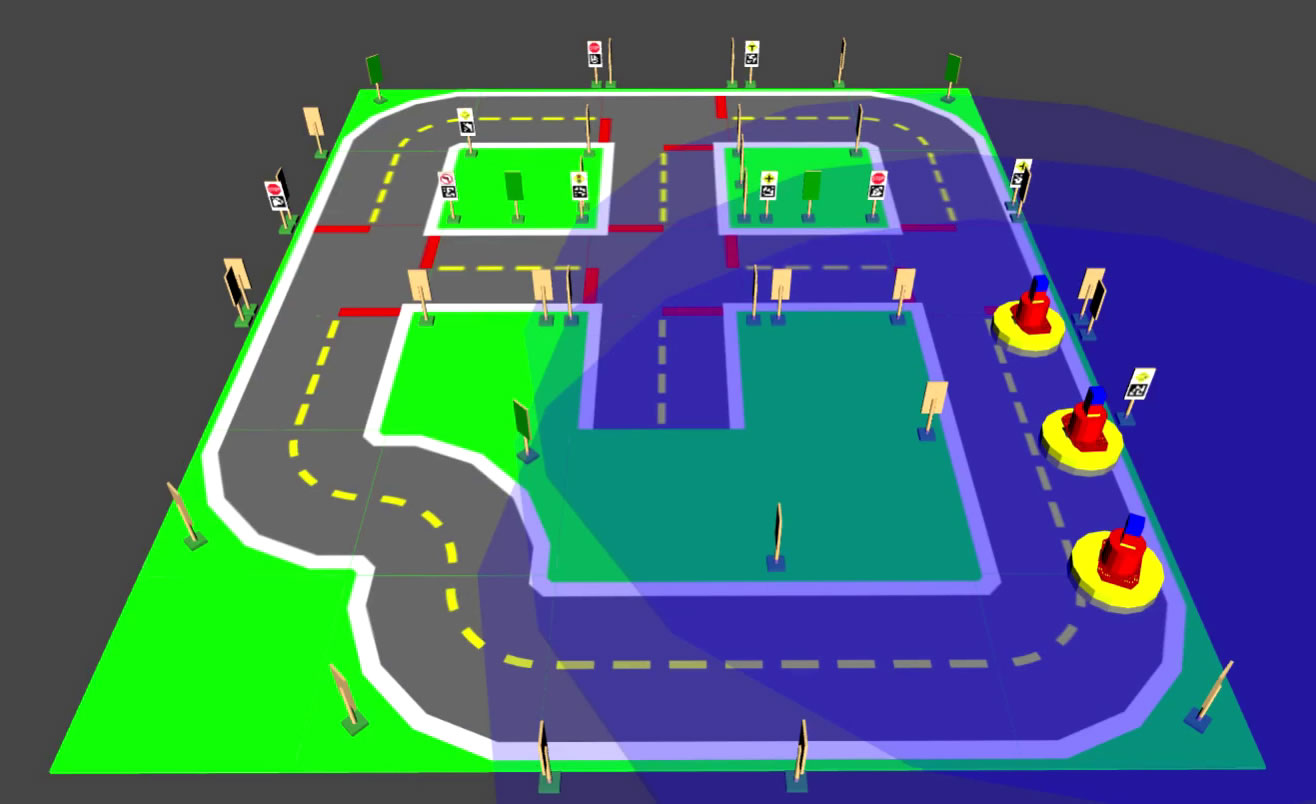
\includegraphics[width=0.48\textwidth]{figures/full-model_viewer.jpg}
    \caption{3D view of Duckietown (no simulation) showing vehicles stopping in line without colliding
    due to an accident located at the North-East 3-way intersection ($POI$).
    The \textit{yellow} circles indicate the position of the vehicles after they stopped.
    The \textit{blue} circles indicate their communication ranges. The \textit{red} cylinders
    indicate the location advertised by the vehicles as \textit{dangerous}. The small \textit{blue boxes}
    indicate that a vehicle is broadcasting messages about known dangerous locations.  \label{fig:3d_viewer_full_model}}
\end{figure}

\section{Background}

For over a decade, the feasibility and applications of communication between autonomous
vehicles have been well defined and studied. The biggest limitations at the time were
network infrastructure and autonomous vehicle technology, but modern networks and technologies
have made communication applications not only feasible but also necessary. 
The applications of communication between autonomous vehicles
span beyond road vehicles and have many practical benefits to other transportation methods
such as trains and planes, but for the purposes of this work the discussion will center
around road vehicles.

The applications of vehicle communication have been well thought out, but one of the key remaining
challenges is implementing a system infrastructure that is able to
effectively deploy such features while keeping in mind the network requirements~\cite{willke2009survey}.
Features such as emergency warnings, collision avoidance, and motion planning
all require different degrees of network speed and reliability that range from
extreme reliability and low latency to more relaxed requirements. With modern networks,
this is becoming less of an issue but is still a key factor we keep in mind while
simulating our communication network.
Recent work has been done to make
the implementation of communication infrastructure much easier by providing a standardized
framework for coordination among a fleet of vehicles~\cite{keila2018}.
This framework would remove
the complications of needing to program individual vehicles and abstracts the global
state of systems controlling deployed vehicles. This will allow users to quickly build
upon single vehicle tasks and deploy concurrent, sequential, or event based tasks
to a fleet of vehicles. This would be extremely useful in road scenarios that require
a large degree of coordination between vehicles in order to safely and efficiently
navigate (e.g. a large pile up of cars on a highway during rush hour).

Improving the efficiency of vehicles on roads (especially highways) has long been a
very obvious application for autonomous vehicle communication~\cite{murray2007recent}.
There has been both recent and established research in this area, in which the question
was essentially how to best model vehicles following one another to
optimize safety and efficiency~\cite{ou2017extended, tanner2003coordination}.
Primary variables considered are velocity
and distance, with findings that support flocking behavior of vehicles where velocities
and distances between vehicles converge to a common value.
In this work, we focus on studying the safety of different communication models.
Specifically, we look at scenarios where traditional methods may be ineffective and propose
a solution that takes into account variables such as network latency and reaction speed.
We present five unique communication features and detail the effectiveness of each one of them
in the context of various safety metrics.
\section{Approach}
\label{sec:solution}

In order to compare the safety of various autonomous vehicle communication networks, we require a vehicle infrastructure that allows customizable communication. To this end, we utilize the Duckietown infrastructure at the Toyota Technical Institute at Chicago [1]. Duckietown is a combination of hardware and software that allows for highly modular autonomous vehicle research. The vehicles use a battery-powered 3-wheeled chassis and are controlled with a Raspberry Pi. They have onboard cameras for lane detection and Wi-Fi devices for communication. Each "Duckiebot" is controlled by the Duckietown software system. This system uses ROS to coordinate all off the concurrent processes on each Duckiebot, which includes processing the camera imagery and sending power to the wheels [2]. We configure and calibrate six Duckiebots for the purposes of this experiment. In order to conduct our experiments, we use a 3-meter wide square which resembles a miniaturized town. The town contains several roads and intersections to allow us to test various scenarios.

In regards to the vehicle communication, we use LCM to send messages between the vehicles [3]. LCM is a multi-platform library that allows simple low-latency messaging. All of the vehicles are connected to a central Wi-Fi device, and subscribe to two common LCM channels. The first channel constantly updates the vehicles with all of the vehicle locations. We later describe the localization process to derive this information. The second channel informs the vehicles of a road-obstruction. These messages are published by the vehicles themselves, and are then selectively ignored by the other vehicles based on the location data. This selective ignoring allows us to emulate the real-world limits of Wi-Fi range. This is an issue for the external validity of our experiments, as the vehicles either accept or reject to recognize a message at a distinct distance. At real-world scale, Wi-Fi packets drop over distance and don't just disappear at a specified range. While we do not have a solution to this, we don't believe it to be very limiting.

Under this framework, we effectively investigate various communication methods. The specific methods in which we are interested are protocols for how safety-affecting data are sent throughout a network of vehicles. More specifically, we observe different messaging protocols for the response of vehicles to the realization of an obstruction. Under these messaging protocols, we compare how the crash rate changes. We will also look at the change in stopping distance from the obstruction.

As a baseline, the first protocol we investigate is Single Messaging. Under this protocol, when a vehicle comes within observation distance of the obstruction, it sends out a single danger message to every vehicle within range and stops. This message contains the location of the danger and the location of the stopped vehicle. Any vehicle that received the message will stop before it reaches either the danger or the stopped vehicle. All other vehicles remain unaware of the danger. This is our baseline protocol as only a single message is sent and so a lot of Wi-Fi bandwidth is wasted. The next protocol is Propagation. Again, the observing vehicle sends a single danger message to all vehicles in range. The vehicle stops, and every vehicle that received the message will stop before it reaches either the danger or the stopped vehicle. These vehicles also retransmit the danger message, which continues for each receiving vehicle. This creates a propagation effect throughout the network of vehicles. The last protocol we investigate is Message Broadcasting. This protocol is the same as Propagation, except that the observing vehicle continuously broadcasts the danger message to all vehicles within range. Again, all receiving vehicles retransmit the message. This should be the safest protocol, but it also requires the most Wi-Fi bandwidth as the message is continuously transmitted. As a control, we compare our findings to a protocol with no communication, in which all vehicles are expected to crash.


\todoinad{FROM HERE}
Emphasize and explain the implementation of three features:
\begin{itemize}
\item message broadcasting
\item message propagation
\item reaction time aware communication
\end{itemize}

Talk about the indoor-GPS that we used.


\todoinad{TO HERE}

References:

[1] Jacopo Tani, et al. ?Duckietown: An Innovative Way to Teach Autonomy? Educational Robotics in the Makers Era Advances in Intelligent Systems and Computing, 2017

[2] Morgan Quigley, et al. ?ROS: an open-source Robot Operating System? 

[3] Huang, Albert, Edwin Olson, David C. Moore. "LCM: Lightweight Communications and Marshalling" 
\section{Evaluation and Results}

We evaluate our communication pipeline on a fleet of robots (i.e., Duckiebots) driving autonomously in a
realistic model of a town called Duckietown~\cite{paull2017duckietown}. Figures~\ref{fig:duckietown}
and~\ref{fig:duckiebot} show respectively our test-bed Duckietown, and one of the Duckiebots used in our
experiments.

\subsection{Implementation}
Duckietown is a robotics educations and outreach effort. For our experiments we use a 3-by-4 meters Duckietown
with three 3-way and one 4-way intersections.
The combination of hardware and software allows for highly modular autonomous vehicles and smart-cities research.
The vehicles used in Duckietown are called Duckiebots (Figure~\ref{fig:duckiebot}) and use a battery-powered 3-wheeled
chassis and are controlled by an on-board Raspberry Pi 3 Model B. Duckiebots feature an on-board camera for lane detection and
a $2.4$GHz b/g/n Wi-Fi module. The Duckietown software stack uses ROS (Robot Operating System)~\cite{quigley2009ros}
as its internal communication protocol, though it does not provide any support or implementation for fleet-level communication.
As for the external communication protocol, we use LCM (Lightweight Communications and Marshalling)~\citep{huang2010lcm}.
LCM is a multi-platform library that allows simple low-latency messaging between processes and devices. All the vehicles are
connected to a central Wi-Fi Access Point.


Self-driving vehicles in the real world can exchange information about locations of interests without any ambiguity since
they all share the same reference frame, that is the geographic coordinate system used by GPS (Global Positioning System) satellites.
Duckietown does not use the standard GPS technology for two reasons: (i) the GPS signal is not available indoors; (ii) the GPS provides
a localization error (about $3-4$ meters) that is bigger than the size of the whole Duckietown.
In order to provide the Duckiebots a GPS-like service, we equipped each Duckiebot with an AprilTag visual fiducial
marker~\cite{olson2011tags} with the normal to the tag orthogonal to the road and pointing to the ceiling of the room.
A camera with wide field-of-view is attached to the ceiling of the room, at the center of the town looking down. This allows
us to estimate the pose of each Duckiebot within Duckietown simply by detecting the fiducial markers and estimating their
poses relative to the camera.
In this setup, the marker-based localization error is about $2cm$, which corresponds to about $4$ meters when scaled to the real world.
The localization service is provided to the Duckiebots via LCM messages with a frequency of about $8Hz$.


\subsection{Experiments}
We test our communication pipeline on a common hazardous situations, that is a car accident at a 3-way
intersection in the case of low visibility conditions. For the remainder of this document we will refer to the location of
the accident (its GPS coordinates) as the \textit{Point of Interest} ($POI$).
In our scenario, after the accident occurred, a number of
vehicles $N$ will approach the same intersection from different directions and with different speed.
We test our model on a variable number of vehicles between $3$ and $6$. We observe consistent
results across all the values of $N$ that we consider.
One experiment starts with $N$ vehicles start moving at the same time and from different locations and
driving towards the $POI$. The experiment ends when all the vehicles stop (either after they crashed
or stopped safely).
In our experiments, due to the lack of visibility, the first vehicle approaching the intersection will inevitably crash
into the damaged vehicle. Immediately after the crash, the communication pipeline of such vehicle takes over.
We are interested in reducing the ratio $C$ of cars colliding with each other, as well as increasing
the average distance $D_p$ from the $POI$ (how far away from the $POI$ a vehicle will stop) and the safety
distance $D_s$, that is the average distance between two consecutive vehicles.

We evaluate the effectiveness of our pipeline by comparing the values of $C$, $D_p$, and $D_s$
with those achieved by the baseline.
In real life scenarios, when no autonomy is involved,
the outcome of such an event heavily depends on the drivers' ability, experience, attention, and
responsiveness~\cite{eby1995analysis} as well as visibility conditions (e.g., lens flare at sunset and
sunrise, fog, occlusions). This makes it hard to define
a baseline to compare against. Although, we can all agree on two points: (i) the worst case (i.e., all approaching
cars crashing) is not unlikely to happen; (ii) the difference between worst and best case scenario is not a mere
number when people's lives are involved. For these reasons, we consider the worst case as a baseline.

\subsection{Technological and Physical limitations}
We are interested in the effect of our model in real life scenarios. In order to reduce the differences between
our lab setup and the real world, we simulate physical effects such as wireless communication range limits,
communication instability due to packets loss, and GPS-based localization latency.
We artificially simulate the wireless communication limit to $\wireless_limit_meter m$ (scaled to real world) by
ignoring all the messages that are sent from a distance that is higher than the limit. Communication instability
is simulated by exchanging information via UDP protocol, that does not attempt re-transmission in case
of lost packets (unlike TCP). We also introduce a $\gps_delay_sec$ second delay between the GPS location
we broadcast to the robots and their actual location.

\subsection{Ablation tests}
As explained in Section~\ref{sec:solution}, our communication pipeline is comprised of five key features.
We believe that these features are fundamental for improving self-driving vehicles' safety via explicit
communication. In order to study the contribution of each feature, we run an ablation test, in which we
run the same number of experiments on a version of our pipeline obtained by disabling one or multiple
features.
In particular, we consider four different models: \textbf{baseline}, \textbf{simple}, \textbf{propagation},
and \textbf{full-model}.

\begin{table}[H]
\centering
\begin{tabular}{|l|r|r|r|r|}
\hline
&
\multicolumn{4}{c|}{\textbf{Model}} \\
\hline
&
	\parbox[t]{2mm}{\multirow{4}{*}{\rotatebox[origin=l]{90}{\textbf{baseline}$\quad\quad\;\;\;$}}}
	&
	\parbox[t]{2mm}{\multirow{4}{*}{\rotatebox[origin=l]{90}{\textbf{simple}$\quad\quad\quad\;\;$}}}
	&
	\parbox[t]{2mm}{\multirow{4}{*}{\rotatebox[origin=l]{90}{\textbf{propagation}$\quad\,$}}}
	&
	\parbox[t]{2mm}{\multirow{4}{*}{\rotatebox[origin=l]{90}{\textbf{full-model$\quad\quad$}}}}
\\
& & & & \\
& & & & \\
& & & & \\
& & & & \\
\textbf{Feature} & & & & \\
\hline
Single message transmission & NO & YES & YES & YES \\
\hline
Message propagation & NO & NO & YES & YES \\
\hline
Message broadcasting & NO & NO & NO & YES \\
\hline
\end{tabular}
\end{table}


We run $\num_test_per_scenario$ tests for each communication model. For a given vehicle, initial position,
speed, and direction are kept unchanged throughout all the tests.

\subsection{Results}

Figure~\ref{fig:collision_ratio} shows the collision ratio observed for different communication models in the
case of $N=3$ vehicles approaching the $POI$. We observe that in the absence of good visual perception
(\textbf{baseline}), as we consider the worst case, the collision rate is $100\%$ as all the vehicles will end up
colliding with each other at the $POI$. By enabling the first vehicle that reaches the $POI$ (and collides) to
warn all the vehicles within the communication range (\textbf{simple}), we found out that on
average, only one vehicle out of $3$ is close enough to receive the message and stop safely. It is worth noting
that any other vehicle entering the communication range after the message was sent will not receive any message
because the vehicle will not keep broadcasting the message. This means that whether or not the vehicles will collide
, strictly depends on their position when the message was generated. A natural extension of this model
would be to allow all the vehicles that received the message to propagate it to other vehicles nearby
(\textbf{propagation} model). We notice that even though the average collision ratio decreases,
the scenario can always degenerate to the case where all vehicles are too far from each other to exchange
messages, hence they will all collide.
Our complete communication pipeline (\textbf{full-model}) features all these communication strategies as well
as a broadcasting mechanism that allow all the vehicles that receive a message to keep publishing it at a frequency
$F$. We empirically found that in our model of town, a frequency of $H=1Hz$ ensures safety while minimizing
the load on the communication channel.

\begin{figure}[t]
    \centering
    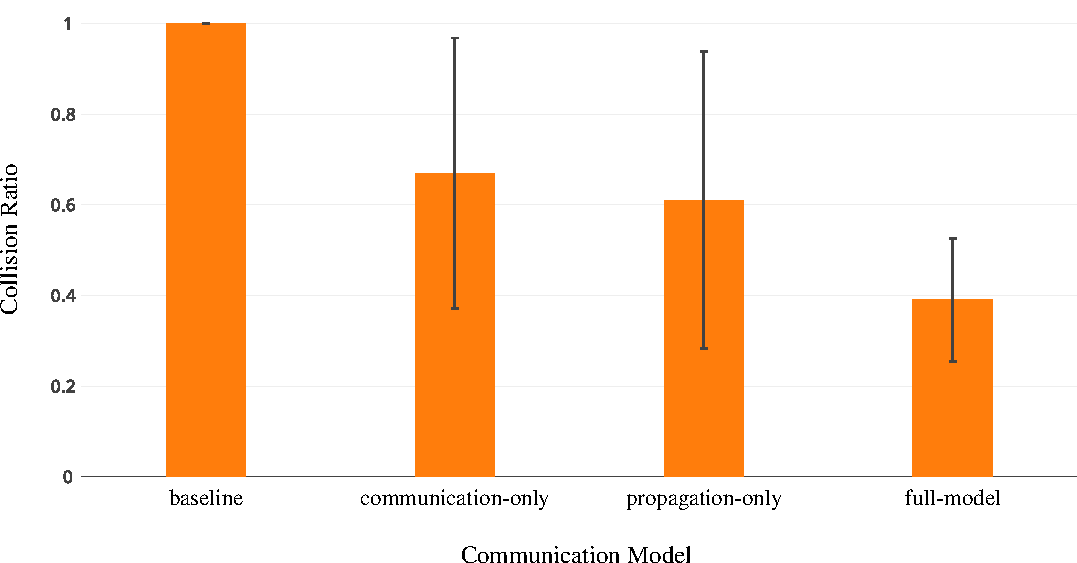
\includegraphics[width=0.48\textwidth, height=0.24\textwidth]{figures/collision_ratio.pdf}
    \caption{Collision ratio ($C$) for different communication models \label{fig:collision_ratio}}
\end{figure}

\begin{figure}[t]
    \centering
    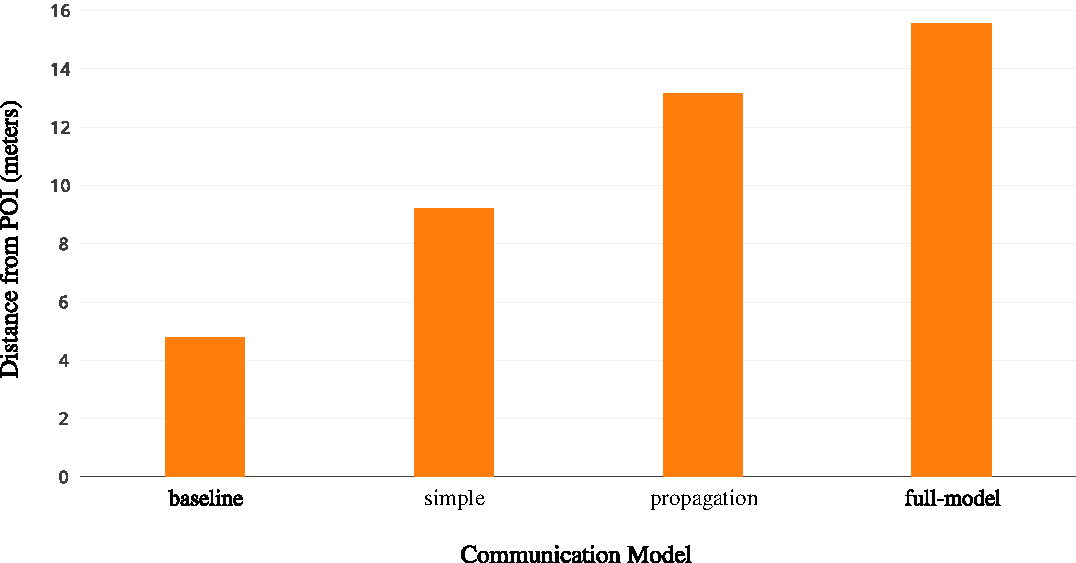
\includegraphics[width=0.48\textwidth, height=0.24\textwidth]{figures/distance_from_POI.pdf}
    \caption{Distance from the $POI$ ($D_p$) for different communication models \label{fig:distance_from_poi}}
\end{figure}

\begin{figure}[t]
    \centering
    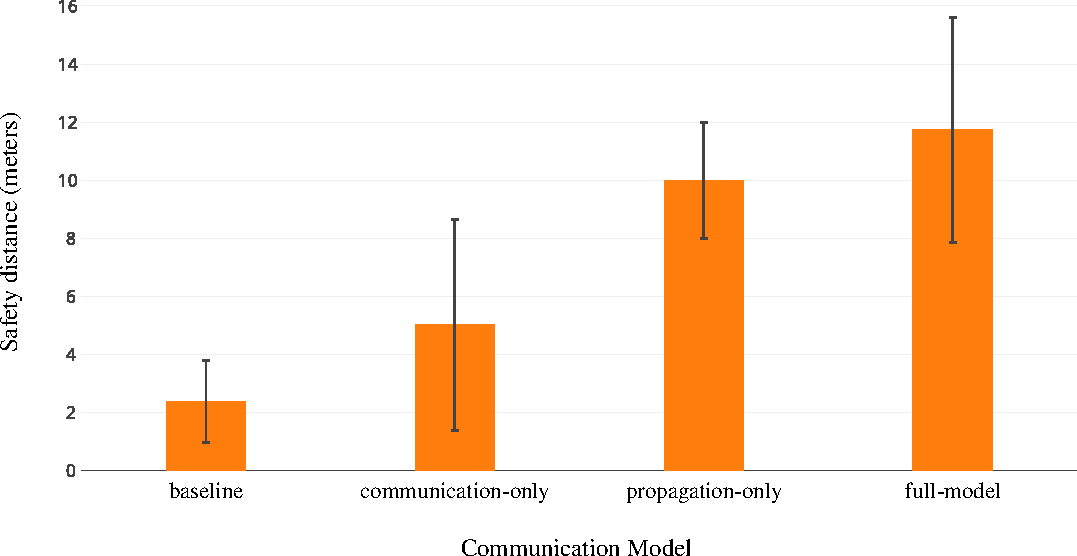
\includegraphics[width=0.48\textwidth, height=0.24\textwidth]{figures/safety_distance.pdf}
    \caption{Safety distance ($D_s$) between two consecutive vehicles \label{fig:safety_distance}}
\end{figure}

Figures~\ref{fig:distance_from_poi} and~\ref{fig:safety_distance} show the average distance
between the $POI$ and the place where the vehicles stopped, and the average distance
between two consecutive vehicles respectively (both scaled to the real world).
The distance $D_p$ is close to $4.5$ meters for the \textbf{baseline} model since all car collide with each
other around the $POI$. The models \textbf{simple} and \textbf{propagation} increase both
$D_p$ and $D_s$ compared to the \textbf{baseline} model, but they fail when vehicles are outside the communication range(s).
The complete pipeline \textbf{full-model} succeed in warning vehicles that enter the communication range(s) later.
Unlike $D_p$, $D_s$ does not depend on the number of vehicles involved in the experiment, hence it
is an absolute indicator of safety. Figure~\ref{fig:3d_viewer_full_model} shows a 3D visualization of Duckietown
in which three Duckiebots stopped in a straight line without colliding into each other
after successfully exchanging messages about an accident located at the North-East 3-way intersection ($POI$).
The \textit{yellow} circles indicate the position of the vehicles after they stopped.
The \textit{blue} circles indicate their communication ranges. The \textit{red} cylinders
indicate the location advertised by the vehicles as \textit{dangerous}.

The proposed communication model achieves a collision ratio reduction of about $\collision_ratio_reduction_perc\%$,
while increasing the distance from the $POI$ and the safety distance between vehicles by a factor of
$3$ and $5$ respectively, compared to the baseline.
It is important to notice that Figure~\ref{fig:collision_ratio} presents a bias of $1/N$ because we assumed that
the first vehicle must collide with the damaged vehicle to detect it. This assumption is necessary to define a
baseline to compare against. Giving the first vehicle to time to perceive the obstacle and stop safely would
raise the question why the others cannot do the same.

\section{Conclusion}

//TODO



%% Use plainnat to work nicely with natbib. 
\bibliographystyle{abbrvnat}
{\small%
	\bibliography{references}%
}

\end{document}